\documentclass{article}
\usepackage[left=3cm, right=3cm, top=2cm, bottom=2cm]{geometry}
\usepackage[colorlinks=true, allcolors=blue]{hyperref}
\usepackage{tikz}
\usepackage{booktabs, multirow} % for borders and merged ranges
\usepackage{soul}% for underlines
\usepackage[table]{xcolor} % for cell colors
\usepackage{changepage,threeparttable} % for wide tables

\title{Data Structures and Algorithms Spring 2024 — Problem Sets}
\author{by Maksim Al Dandan}

\begin{document}
\maketitle{\section*{Week 13. Problem set}}

\section{Task 1}
\subsection{Statement}

Run the Floyd-Warshall algorithm~\cite[\S 23.2]{cormen} on the following graph. Use the alphabetic order of vertices. Show the state of distance matrix \(D\) after each iteration of outer loop in the algorithm. Since the graph has \(5\) vertices, you must provide five \(5 \times 5\) matrices in your answer. No justification is required.
        
        \begin{center}
            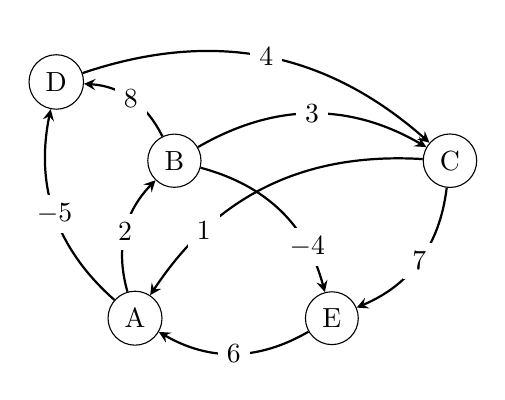
\begin{tikzpicture} [
                    thick,
                    every node/.style={fill=white},
                    vertex/.style={thin, draw, circle},
                ]
                \path {
                    (+0.0, +0.0) node [vertex] (A) {A}
                    (+0.5, +2.0) node [vertex] (B) {B}
                    (+4.0, +2.0) node [vertex] (C) {C}
                    (-1.0, +3.0) node [vertex] (D) {D}
                    (+2.5, +0.0) node [vertex] (E) {E}
                };
                \draw[-stealth] (A) to [bend left]  node [midway]   {\(2\)}  (B);
                \draw[-stealth] (A) to [bend left]  node [midway]   {\(-5\)} (D);
                \draw[-stealth] (B) to [bend left]  node [midway]   {\(3\)}  (C);
                \draw[-stealth] (B) to [bend right] node [midway]   {\(8\)}  (D);
                \draw[-stealth] (B) to [bend left]  node [near end] {\(-4\)} (E);
                \draw[-stealth] (C) to [bend right] node [near end] {\(1\)}  (A);
                \draw[-stealth] (C) to [bend left]  node [midway]   {\(7\)}  (E);
                \draw[-stealth] (D) to [bend left]  node [midway]   {\(4\)}  (C);
                \draw[-stealth] (E) to [bend left]  node [midway]   {\(6\)}  (A);
            \end{tikzpicture}
        \end{center}

\subsection{Solution}

\textbf{Initial matrix}
\begin{table}[!htp]\centering
    \scriptsize
    \begin{tabular}{lrrrrrr}\toprule
    &\textbf{A} &\textbf{B} &\textbf{C} &\textbf{D} &\textbf{E} \\\midrule
    \textbf{A} &0 &2 &$\infty$ &-5 &$\infty$ \\
    \textbf{B} &$\infty$ &0 &3 &8 &-4 \\
    \textbf{C} &1 &$\infty$ &0 &$\infty$ &7 \\
    \textbf{D} &$\infty$ &$\infty$ &4 &0 &$\infty$ \\
    \textbf{E} &6 &$\infty$ &$\infty$ &$\infty$ &0 \\
    \bottomrule
    \end{tabular}
\end{table}

\textbf{Matrix after 1-st iteration}
\begin{table}[!htp]\centering
    \scriptsize
    \begin{tabular}{lrrrrrr}\toprule
    &\textbf{A} &\textbf{B} &\textbf{C} &\textbf{D} &\textbf{E} \\\midrule
    \textbf{A} &0 &2 &$\infty$ &-5 &$\infty$ \\
    \textbf{B} &$\infty$ &0 &3 &8 &-4 \\
    \textbf{C} &1 &3 &0 &-4 &7 \\
    \textbf{D} &$\infty$ &$\infty$ &4 &0 &$\infty$ \\
    \textbf{E} &6 &8 &$\infty$ &1 &0 \\
    \bottomrule
    \end{tabular}
\end{table}

\newpage

\textbf{Matrix after 2-nd iteration}
\begin{table}[!htp]\centering
    \scriptsize
    \begin{tabular}{lrrrrrr}\toprule
    &\textbf{A} &\textbf{B} &\textbf{C} &\textbf{D} &\textbf{E} \\\midrule
    \textbf{A} &0 &2 &5 &-5 &-2 \\
    \textbf{B} &$\infty$ &0 &3 &8 &-4 \\
    \textbf{C} &1 &3 &0 &-4 &-1 \\
    \textbf{D} &$\infty$ &$\infty$ &4 &0 &$\infty$ \\
    \textbf{E} &6 &8 &11 &1 &0 \\
    \bottomrule
    \end{tabular}
\end{table}

\textbf{Matrix after 3-rd iteration}
\begin{table}[!htp]\centering
    \scriptsize
    \begin{tabular}{lrrrrrr}\toprule
    &\textbf{A} &\textbf{B} &\textbf{C} &\textbf{D} &\textbf{E} \\\midrule
    \textbf{A} &0 &2 &5 &-5 &-2 \\
    \textbf{B} &4 &0 &3 &-1 &-4 \\
    \textbf{C} &1 &3 &0 &-4 &-1 \\
    \textbf{D} &5 &7 &4 &0 &3 \\
    \textbf{E} &6 &8 &11 &1 &0 \\
    \bottomrule
    \end{tabular}
\end{table}

\textbf{Matrix after 4-th iteration}
\begin{table}[!htp]\centering
    \scriptsize
    \begin{tabular}{lrrrrrr}\toprule
    &\textbf{A} &\textbf{B} &\textbf{C} &\textbf{D} &\textbf{E} \\\midrule
    \textbf{A} &0 &2 &-1 &-5 &-2 \\
    \textbf{B} &4 &0 &3 &-1 &-4 \\
    \textbf{C} &1 &3 &0 &-4 &-1 \\
    \textbf{D} &5 &7 &4 &0 &3 \\
    \textbf{E} &6 &8 &5 &1 &0 \\
    \bottomrule
    \end{tabular}
\end{table}

\textbf{Matrix after 5-th iteration}
\begin{table}[!htp]\centering
    \scriptsize
    \begin{tabular}{lrrrrrr}\toprule
    &\textbf{A} &\textbf{B} &\textbf{C} &\textbf{D} &\textbf{E} \\\midrule
    \textbf{A} &0 &2 &-1 &-5 &-2 \\
    \textbf{B} &2 &0 &1 &-3 &-4 \\
    \textbf{C} &1 &3 &0 &-4 &-1 \\
    \textbf{D} &5 &7 &4 &0 &3 \\
    \textbf{E} &6 &8 &5 &1 &0 \\
    \bottomrule
    \end{tabular}
\end{table}

\section{Task 2}
\subsection{Statement}

Provide a graph with exactly \(4\) vertices (A, B, C, D) and \(4\) weighted edges, such that Dijkstra's algorithm~\cite[\S 22.3]{cormen} does \textbf{not} give a correct shortest distance for at least one vertex:
        
        \begin{enumerate}
            \item Provide the graph (the graph must be rendered in a clear way, text representation is not
                enough); Weights must be (small) integers.
                
            \item Provide the result of Dijkstra's algorithm for each vertex: any shortest path \textbf{and} corre-
                sponding total weight;
                
            \item Provide the correct shortest path and corresponding total weight for each vertex;
                
            \item Explain why Dijkstra's algorithm did not provide the correct answer (specifically for your
                example, generic justification is not accepted).
        \end{enumerate}

\subsection{Solution}

\textbf{Graph with 4 vertices and 4 weighted edges}

\begin{center}
    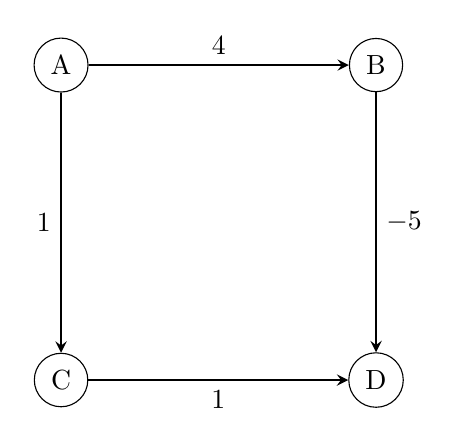
\begin{tikzpicture} [
            thick,
            every node/.style={fill=white},
            vertex/.style={thin, draw, circle},
        ]
        \path {
            (+0.0, +0.0) node [vertex] (A) {A}
            (+4.0, +0.0) node [vertex] (B) {B}
            (+0.0, -4.0) node [vertex] (C) {C}
            (+4.0, -4.0) node [vertex] (D) {D}
        };
        \draw[-stealth] (A) -- node [midway, above] {\(4\)} (B);
        \draw[-stealth] (A) -- node [midway, left]  {\(1\)} (C);
        \draw[-stealth] (C) -- node [midway, below] {\(1\)} (D);
        \draw[-stealth] (B) -- node [midway, right] {\(-5\)} (D);
    \end{tikzpicture}
\end{center}

\textbf{Result of Dijkstra's algorithm for each vertex}

\begin{itemize}
    \item From A to B: Path A-B with total weight 4.
    \item From A to C: Path A-C with total weight 1.
    \item From A to D: Path A-B-D with total weight -1 (Incorrect due to negative weight).
\end{itemize}

\textbf{Correct shortest path and corresponding total weight for each vertex}

\begin{itemize}
    \item From A to B: Path A-B with total weight 4.
    \item From A to C: Path A-C with total weight 1.
    \item From A to D: Path A-C-D with total weight 5.
\end{itemize}

\textbf{Explanation} \\

Dijkstra's algorithm did not provide the correct answer for the vertex D because it cannot handle graphs with negative weight edges properly. In this example, the algorithm prematurely concludes that the shortest path to D is through B because it does not revisit vertices with updated distances once they have been marked as visited. This leads to the incorrect assumption that the path A-B-D is shorter than it actually is, ignoring the fact that the path A-C-D is the correct shortest path when considering all edges, including those with negative weights.

\section{Task 3}
\subsection{Statement}

Since Dijkstra's shortest paths algorithm~\cite[\S 22.3]{cormen} does not work with negative edges in general, consider an algorithm that, for a given graph \(G\), if it has a negative edge, finds the minimum edge in \(G\) with the weight \((-W)\) and adds \((+W)\) to all edges in the original graph, resulting in a new graph \(G^{+W}\). Then the modified algorithm runs Dijkstra's algorithm on \(G^{+W}\). Are the resulting shortest paths in \(G^{+W}\) also shortest in \(G\)? If yes, prove it. If no, provide a concrete counterexample and a justification.

\subsubsection{Solution}

\textbf{Answer:} No, the resulting shortest paths in \(G^{+W}\) are not necessarily the shortest paths in the original graph \(G\).

\textbf{Counterexample:}

Consider a graph \(G\) with three vertices \(A\), \(B\), and \(C\), and three edges: \(A \rightarrow B\) with weight \(-2\), \(B \rightarrow C\) with weight \(2\), and \(A \rightarrow C\) with weight \(1\).

\begin{center}
    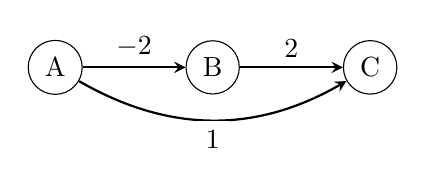
\begin{tikzpicture} [
            thick,
            every node/.style={fill=white},
            vertex/.style={thin, draw, circle},
        ]
        \path {
            (+0.0, +0.0) node [vertex] (A) {A}
            (+2.0, +0.0) node [vertex] (B) {B}
            (+4.0, +0.0) node [vertex] (C) {C}
        };
        \draw[-stealth] (A) -- node [midway, above] {\(-2\)} (B);
        \draw[-stealth] (B) -- node [midway, above] {\(2\)} (C);
        \draw[-stealth] (A) to [bend right] node [midway, below] {\(1\)} (C);
    \end{tikzpicture}
\end{center}

In \(G\), the shortest path from \(A\) to \(C\) is directly from \(A\) to \(C\) with a total weight of \(1\).

Now, we find the minimum edge weight, which is \(-2\), and add \(2\) to all edges in \(G\) to get \(G^{+2}\):

\begin{center}
    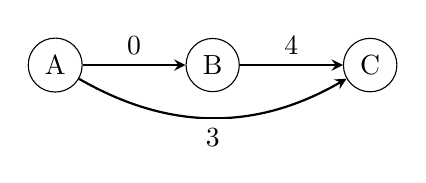
\begin{tikzpicture} [
            thick,
            every node/.style={fill=white},
            vertex/.style={thin, draw, circle},
        ]
        \path {
            (+0.0, +0.0) node [vertex] (A) {A}
            (+2.0, +0.0) node [vertex] (B) {B}
            (+4.0, +0.0) node [vertex] (C) {C}
        };
        \draw[-stealth] (A) -- node [midway, above] {\(0\)} (B);
        \draw[-stealth] (B) -- node [midway, above] {\(4\)} (C);
        \draw[-stealth] (A) to [bend right] node [midway, below] {\(3\)} (C);
    \end{tikzpicture}
\end{center}

In \(G^{+2}\), the shortest path from \(A\) to \(C\) is now \(A \rightarrow B \rightarrow C\) with a total weight of \(4\). However, when we subtract the added weight (\(2 \times 2 = 4\)) from this total, we get \(0\), which is not the shortest path weight in the original graph \(G\).

\textbf{Justification:}

The process of adding a constant weight to all edges in a graph with negative edges can alter the relative weights of different paths. While this transformation makes all edges non-negative, allowing Dijkstra's algorithm to be applied, it does not preserve the original shortest path properties of the graph. This is because the added weight disproportionately affects shorter paths less than longer paths, potentially making a longer path seem shorter after the transformation. Therefore, the resulting shortest paths in \(G^{+W}\) are not guaranteed to be the shortest paths in the original graph \(G\).

\begin{thebibliography}{.week-13.}
    \bibitem[Cormen]{cormen} T. H. Cormen, C. E. Leiserson, R. L. Rivest and C. Stein.\ \emph{Introduction to Algorithms,
        Fourth Edition}. The MIT Press 2022
\end{thebibliography}
\end{document}
